\section{Judas}
\label{res:Judas}

\subsection{Result Setup}

All the tests for Judas were run on local servers belonging to \acrshort{cgf}. The details are all listed in the table below. \\


\begin{table}[h]
\centering
\begin{tabular}{|l|l|}
\hline
\textbf{Unit} & \textbf{Desc}         \\ \hline
Os            & Ubuntu Linux          \\ \hline
Processor     & Intel i9-9940X @ 4GHz \\ \hline
Ram           & 126GB                 \\ \hline
GPU           & NVIDIA RTX 2080TI     \\ \hline
VRAM          & 11GB                  \\ \hline
Gpu Cores     & 4352                  \\ \hline
\end{tabular}
\label{tab:cgfspecs}
\caption{Specs for our machine running our code}
\end{table}

\subsection{Experiment: HDF5 file processing and resampling}

In this experiment, we will be processing $n$ amount of \acrshort{hdf5} files with $p$ processes, from the point of reading raw data gathered by \acrshort{cgf} from the OptoDAS, through pre-processing, resampling the signals and denoising the result. This will give an accurate view of what needs to happen from rawdata until they are ready to be trained on different \acrshort{ml} or \acrshort{dl} models. \\

We will be resampling the signals to $100Hz$ from $500Hz$, and the Channel ROI will be 250m. We will be utilizing 1, 2, 4 and 8 processes, and use of a different amount of \acrshort{das} data ranging from 10 seconds until 1 hour of \acrshort{das} data.



\begin{figure}[htbp]
\centering
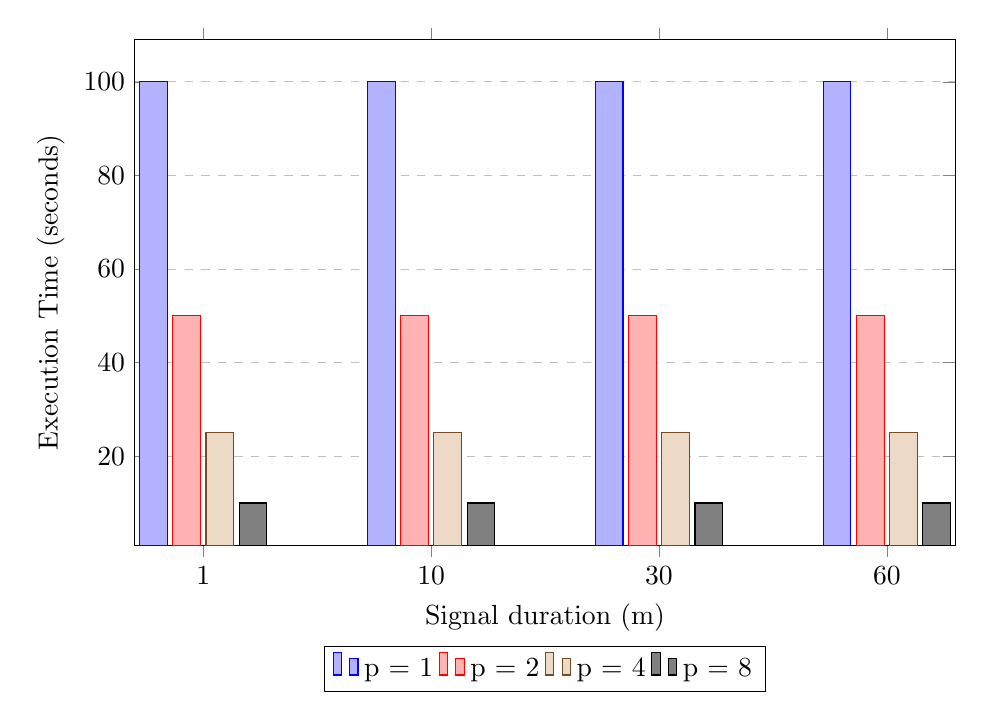
\begin{tikzpicture}
\begin{axis}[
    ylabel={Execution Time (seconds)},
    xlabel={Signal duration (m)},
    xticklabels={1,10, 30, 60},
    xtick={1,10,30,60},
    legend pos=north west,
    ymajorgrids=true,
    grid style=dashed,
    width=12cm,
    height=8cm,
    bar width=10pt,
    ybar,
    legend style={at={(0.5,-0.20)},
    anchor=north,legend columns=-1},
    symbolic x coords={1, 10, 30, 60},
]
\addplot coordinates {(1,100)(10,100)(30,100)(60,100) };
\addplot coordinates {(1,50) (10,50) (30,50) (60,50) };
\addplot coordinates {(1,25) (10,25) (30,25) (60,25) };
\addplot coordinates {(1,10) (10,10) (30,10) (60,10) };
\legend{p = 1, p = 2, p = 4, p = 8}
\end{axis}
\end{tikzpicture}
\caption{Execution times for different problem sizes and process counts}
\label{fig:judas-benchmark}
\end{figure}

As we can see.

\begin{figure}[htbp]
\centering
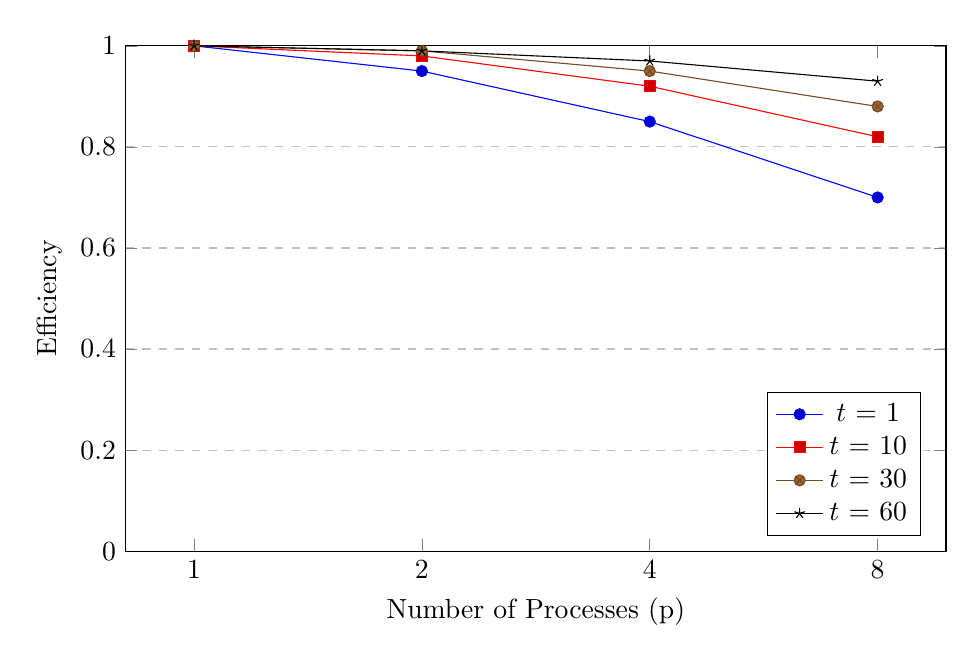
\begin{tikzpicture}
\begin{axis}[
    ylabel={Efficiency},
    xlabel={Number of Processes (p)},
    xticklabels={1,2,4,8},
    xtick={1,2,3,4},
    legend pos=south east,
    ymajorgrids=true,
    grid style=dashed,
    width=12cm,
    height=8cm,
    ymax=1,
    ymin=0,
]
\addplot coordinates {(1,1) (2,0.95) (3,0.85) (4,0.70)};
\addplot coordinates {(1,1) (2,0.98) (3,0.92) (4,0.82)};
\addplot coordinates {(1,1) (2,0.99) (3,0.95) (4,0.88)};
\addplot coordinates {(1,1) (2,0.99) (3,0.97) (4,0.93)};
\legend{$t$ = 1, $t$ = 10, $t$ = 30, $t$ = 60}
\end{axis}
\end{tikzpicture}
\caption{Efficiency for different problem sizes and process counts. $m$ is the amount of minutes of data we want to process.}
\label{fig:efficiency}
\end{figure}